\chapter{Realisierung des Clients als Web Applikation}
\label{cha:web-app}
In diesem Kapitel wird die Implementierung des Clients als Web-Applikation beschrieben. Hierbei wird genauer auf die verschiedenen Design-Entscheidungen und genutzten Techniken näher eingegangen. 
\section{Definition einer Single Page Application}
\label{sec:Definition-SPA}
Die Web-Applikation wurde als \ac{SPA} implementiert. Bei dieser Art der Webanwendung wird die Verarbeitung von Anfragen vom Server auf die Clients verschoben. Die daraus entstehende Anwendung benutzt nur wenige statische Hauptseiten, um den Inhalt darzustellen. Alle dynamischen Inhalte der Seite werden nachträglich per \ac{AJAX}-Requests hinzugeladen.  Hierbei wird die Verarbeitung der nachgeladenen Daten auf dem Client durchgeführt und anschließend in die vorhandene \textit{\ac{HTML}}-Struktur übernommen, wobei der Grad der Autonomie des Clients vom genutzten Framework abhängt. Diese Auslagerung der Verarbeitung begünstigt die Nutzung des \ac{REST}ful Web Services (siehe Kapitel \ref{cha:server-impl}), welcher die Daten liefert, die die \ac{SPA} dann verarbeiten kann. Daraus ergibt sich, dass nur eine lose Verbindung zum Web Server besteht, sodass nur die wenigen statischen Seiten und deren eingebundene Skripte abgerufen werden müssen. Die sonstige Kommunikation besteht nur noch zwischen der \ac{SPA} und dem Web Service.\footcite[S. 31f.]{book:AngularJs:Steyer2015} \\
Im Laufe dieses Kapitels wird noch darauf eingegangen, wie auch diese beiden Verbindungen durch geeignete Techniken bis auf ein Mindestmaß reduziert wurden.
\section{AngularJS}
\label{sec:AngularJS}
Zur Umsetzung der \ac{SPA} wurde das quelloffene Framework \textit{AngularJS} von \textit{Google} gewählt, welches sich immer größerer Popularität erfreut.\footcite{online:angularjs-popularity}\footcite[S. 33]{book:AngularJs:Steyer2015} Es bietet alle Möglichkeiten, um eine Web-Anwendung als weitestgehend autonomen \gls{Fat-Client} zu implementieren. Dadurch wird die Möglichkeit geschaffen, eine Applikation zu entwickeln, welche selbst dann akzeptabel reagiert, wenn ein aufrufendes Endgerät keine Verbindung zum Internet besitzt. Hierzu stellt es zusätzliches \gls{Markup} bereit, welches zu Laufzeit interpretiert und ausgeführt wird. Die dazu nötigen Komponenten von AngularJS und deren Einsatz werden nachfolgend genauer erläutert.

\subsection{Abgrenzung des Begriffs: Komponente}
Wenn in diesem Kapitel der Begriff Komponente verwendet wird, ist eine abgeschlossene, logische Einheit im AngularJS-Umfeld gemeint. Auf einige dieser Komponenten, wie Services und Controller, wird im späteren Verlauf dieses Kapitels detaillierter eingegangen. AngularJS nutzt den Begriff des \textit{Modules} als einen Container für verschiedene Komponenten\footcite{online:angular:module}. 
\subsection{Dependency Injection}
\label{ssec:SPA-Dependency-Injection}
AngularJS wurde so konstruiert, dass zu jedem Zeitpunkt eine gute Testbarkeit gewährleistet ist.\footcite{online:angularjs:testability} Aus diesem Grund setzt AngularJS für die Verbindung von verschiedenen Funktionen auf \textit{Dependency Injection}. \\ 
Hierbei werden beim Ausführen einer Funktion die genutzten Parametern geprüft. Gibt es eine bekannte Komponente, die den gleichen Namen wie der geforderte Parameter besitzt, erzeugt AngularJS ein Objekt diese Komponente und übergibt dieses an die Funktion. Dieser Vorgang wird rekursiv durchgeführt, sodass ebenfalls Dependency Injection für die Erzeugung der jeweiligen Parameter-Objekte benutzt wird.\footcite{online:angularjs:dependency-injection}
\subsection{Services}
\label{ssec:SPA-Services}
\textit{Services} sind abgeschlossene Komponenten, welche bestimmte Funktionalitäten kapseln und bereitstellen. AngularJS bietet neben der Möglichkeit, eigene Services zu erstellen, eine eigene Auswahl, um verschiedene wiederkehrende Aufgaben durchzuführen. Dabei sind die Services von AngularJS immer mit dem Präfix \textit{\$} versehen. Einer der wichtigsten Services für die Umsetzung dieser Arbeit war beispielsweise \textit{\$http}. Dieser stellt Funktionen bereit, welche zur Kommunikation eines Web Services mittels \ac{HTTP} benötigt werden. \\
Services können von Controllern (siehe \ref{ssec:SPA-MVC}) verwendet werden, um Daten zu erhalten und an die Oberfläche weiterzugeben. Hierbei verwenden Sie Dependency Injection, um auf einen \textit{Service} zuzugreifen, wobei nur beim ersten Zugriff ein neues Objekt erzeugt wird (\gls{Singleton}-Muster). Fordert eine weitere Komponente ein Objekt des Services an, wird das bereits erstellt Objekt zurückgegeben. \footcite{online:angular:services}
\subsection{Promises}
\label{ssec:SPA-Promises}
Im letzten Abschnitt wurde der Service \textit{\$http} angesprochen (siehe \ref{ssec:SPA-Services}), welcher Methoden zur Kommunikation mit einem \ac{REST}ful Web Service bereitstellt. Würde diese Kommunikation synchron ausgeführt werden, würde diese AngularJS bis zum Erhalt der Antwort blockieren, da \textit{\gls{Javascript}} immer nur in einem Thread ausgeführt wird\footcite{online:javascript:single-threaded}. Deshalb wurde das Prinzip der \textit{Promises} eingeführt. Dies erlaubt die Abarbeitung von asynchronem Code, indem beim Aufruf einer asynchron abzuarbeitenden Methode ein Promise-Objekt zurückgegeben wird. Dieses repräsentiert ein Versprechen über einen späteres Ergebnis. Auf dieses Ergebnis kann mit den Methoden \textit{then} und \textit{catch} reagiert werden. \\ 
\textit{Then} wird nach erfolgreicher Abarbeitung der asynchronen Methode ausgeführt. Tritt bei der Verarbeitung ein Fehler auf, wird die \textit{catch}-Methode ausgeführt. Da diese beiden Methoden jeweils selber Promise-Objekte zurückgeben, ist ein verketten der Aufrufe möglich. 
Die Nutzung von Promisses ist im Module \textit{\$q} gekapselt, welches sich an dem Projekt \textit{q}\footcite{online:doc_q} orientiert.\footcite{online:angular:module:q}\footcite[S. 211ff]{book:AngularJs:Steyer2015}
\subsection{MVC}
\label{ssec:SPA-MVC}
AngularJS nutzt das Architektur-Muster \textit{\ac{MVC}} um Datenbeschaffung bzw. -haltung, Datenverarbeitung und Datenpräsentation strikt zu trennen.\footcite[S.34]{book:AngularJs:Steyer2015} \\ 
Zur Beschaffung werden entweder Services, welche per Dependency Injection hinzugeladen werden, benutzt oder Funktionen zur Erzeugung von Model-Objekte erstellt, welche mit Konstruktoren aus dem objektorientierten Umfeld verglichen werden können. \\
Die so erhaltenen Datenstrukturen können von Controllern aufgerufen werden. Dabei handelt es sich um Komponenten, welche von AngularJS zur Anreicherung eines bestimmten \gls{Markup}-Blocks aufgerufen werden. Ihre Aufgabe ist es, die für die Oberfläche benötigten Daten zu besorgen, diese aufzubereiten und sie an die View weiterzugeben. Das Code-Beispiel \ref{lst:SPA-controller-navigation} zeigt den Aufbau einer Controller-Komponente, welche Daten für die Navigationsleiste bereitstellt\footcite{online:angular:controller}.
\lstinputlisting[caption=Controller für die Navigationsleiste, label=lst:SPA-controller-navigation, style=htmlcssjs]{content/listings/indexcontroller.js}
Hierbei ist zu sehen, wie mittels Dependency Injection die benötigten Komponenten für die Funktion bereitgestellt werden (siehe Code-Beispiel \ref{lst:SPA-controller-navigation}  Zeile \ref{line:controller:dependency-injection}). Interessant ist dabei besonders die Komponente \textit{\$scope}. Diese wird verwendet, um Daten zwischen dem Controller und der View (in dem Fall: der statischen HTML-Seite) auszutauschen (siehe Code-Beispiel \ref{lst:SPA-controller-navigation} Zeile \ref{line:controller:scope}ff.)\footcite{online:angular:scopes}. Dabei stellt AngularJS Funktionen bereit, um diesen Austausch bidirektional durchzuführen. Somit können beispielsweise Daten, welche ein Nutzer in ein Textfeld eingibt, im Controller weiterverarbeitet werden.\\
Die Benutzung der durch den \textit{\$scope} bereitgestellten Variablen wird im Code-Beispiel \ref{lst:SPA-navigation} gezeigt.\\
\lstinputlisting[caption=Navigation der Hauptseite erweitert um AngularJS-Markup, label=lst:SPA-navigation, style=htmlcssjs]{content/listings/Index.html}
Über das Attribut \textit{data-ng-controller} (siehe Code-Beispiel \ref{lst:SPA-navigation} Zeile \ref{line:indexHtml:controller}) wird ausgesagt, dass dieser \textit{div}-Block durch die Controller-Funktion \textit{indexController} bearbeitet wird. Nur in diesem Geltungsbereich kann auf die Eigenschaften des Controllers zugegriffen werden. \\
Hierbei gibt es verschiedene Möglichkeiten, die Daten des Controllers zu benutzten: 
\begin{itemize}
\item \textbf{Nutzung in Direktiven}\\
AngularJS stellt Direktiven bereit, welche die Darstellung der Webseite beeinflussen. Dies zeigt sich in Zeile \ref{line:indexHtml:Nutzung_Direktive}. Die Direktive \textit{ng-hide} wird benutzt, um dynamisch \ac{HTML}-Elemente auszublenden. Für die Entscheidung, ob das zugehörige \textit{li}-Element ausgeblendet werden soll, wird die Variable \textit{onlineStatus} aus dem \textit{\$scope} des Controllers abgefragt. Ändert sich die Variable im Controller, wird die Direktive neu ausgewertet\footcite{online:angular:diretive}.
\item \textbf{Ausgabe des Wertes}\\
Der Wert einer Variable kann direkt ausgegeben werden. Dies wird in Zeile \ref{line:indexHtml:Nutzung_Variable} gezeigt. Damit AngularJS erkennt, dass eine \textit{\$scope}-Variable ausgegeben werden soll, muss diese von zwei geschweiften Klammern umgeben sein.
\item \textbf{Zugriff auf Methoden}\\
In Zeile \ref{line:indexHtml:Nutzung_Methode} wird eine Direktive benutzt, um aus der View heraus eine im \textit{\$scope} definierte Funktion aufzurufen.
\end{itemize}
\subsection{Routing}
\label{ssec:SPA-Routing}
Damit das \gls{Markup} nicht schnell durch die Nutzung von zusätzlichen Direktiven überladen wird, bietet AngularJS das Module \textit{\$route} zur Implementierug von Routing an. Hierbei wird durch die Direktive \textit{ng-view} ein Block-Element (z.B. ein \textit{div}-Element) als View-Container definiert. Dieser wird abhängig von der aufgerufenen URL mit unterschiedlichen Inhalten befüllt. Das Code-Beispiel \ref{lst:SPA-routing} zeigt solch eine Routing-Konfiguration. 
\lstinputlisting[caption=Routing mit AngularJS, label=lst:SPA-routing, style=htmlcssjs]{content/listings/routing.js}
Stimmt eine Route überein, wird der konfigurierte Controller aufgerufen. Dessen Scope wird nach der Abarbeitung an die definierte View weitergegeben. Die Views sind hierbei \ac{HTML}-Dateien mit \gls{Markup}-Schnipsel, die innerhalb des View-Containers erzeugt werden. Diese \gls{Markup}-Schnipsel liegen ebenfalls auf dem Server. 
\section{Umsetzung}
\label{sec:SPA-Umsetzung}
Durch die Nutzung der vorgestellten Komponenten und eines Tutorials\footcite{online:Created_SPA} war es möglich, einen Prototyp umzusetzen, welcher die grundlegenden Anforderungen, die in Kapitel \ref{cha:architektur} definiert wurden, erfüllt. Nachfolgend werden einige Teilaspekte im Zusammenhang mit der Implementierung näher beleuchtet.
\subsection{Layout mit Twitter Bootstrap}
\label{ssec:SPA-twitter-bootstrap}
Zur Erstellung einer Oberfläche wurde vollständig auf das quelloffene \linebreak \ac{CSS}-Framework \textit{Bootstrap} von \textit{Twitter} gesetzt. Dies ist unter dem Aspekt designet, einmal definiertes \ac{CSS} auf allen Endgeräten eine natürliche und gut nutzbare Anwendung entsteht.\footcite{online:get-bootstrap} Dies liegt daran, dass Bootstrap es erlaubt, unter Nutzung eines integrierten Grid-Systems, eine -\gls{responsiv}e Applikation zu erstellen.\\
Durch den großen Umfang des Frameworks und da im ersten Schritt nur ein Prototyp erzeugt werden sollte, war es möglich, alle Anforderungen in die Web-Applikation zu integrieren, ohne, dass weitere Implementierung von \ac{CSS} nötig war.

\subsection{Herausforderungen durch das statusloses Protokoll HTTP}
\label{ssec:statusloses-http}
Da \ac{HTTP} ein statusloses Protokoll ist, ist es nicht ohne Weiteres möglich, ein einmal abgerufenes \textit{Access-Token} wiederzuverwenden. Um dies dennoch zu erreichen, wurde Service \textit{authFactory} entwickelt, welcher  das ein- und ausloggen verwaltet. Hierbei wird unter Zuhilfenahme der \textit{LocalStorage}-\ac{API} ein erhaltenes \textit{Access-Token} mit dem Nutzernamen und dem Ablaufdatum persistiert. Ist dieser Datensatz vorhanden und das Ablaufdatum noch nicht erreicht, gilt der Nutzer als angemeldet und kann auf seine Trainingspläne zugreifen. \\
Gleichzeitig wird für die Verwaltung von Inhalt, welchen nur authentifizierte Nutzer abrufen können, eine weitere Komponente namens \textit{Interceptor} benutzt. Dies ist ein spezieller Service, der eng mit dem \textit{\$http}-Service verbunden ist.\footcite{online:angular:interceptor} Mit dem Interceptor ist es möglich, eine Request kurz vor- und eine Response direkt nach Erhalt einzusehen und gegebenenfalls darauf zu reagieren. Diese Technik wird verwendet, um vor dem Absenden eines Requests den \textit{authorizsation}-Header zu setzen, falls ein Access-Token vorhanden ist. \\ 
Die Response ist wegen des eingehenden Statuscodes interessant: Wenn der Web Service mit \textit{401 (Unauthorised)} antwortet, ist der Nutzer nicht angemeldet. Daraufhin wird ein möglicher Datensatz mit einem Access-Token gelöscht und der Nutzer wird auf die Login-Seite umgeleitet\footcite{online:Created_SPA}. 

\subsection{Online-Check}
\label{ssec:Online-Check}
Der Nutzer soll eine visuelle Rückmeldung darüber bekommen, ob die Applikation momentan eine Verbindung zum Web Service aufbauen kann oder nicht. Dafür wurde der im Quellcode-Beispiel \ref{lst:SPA-controller-navigation} gezeigte Controller um einen Online-Check erweitert. Darin ruft die Anwendungen in einem 5 Sekunden-Intervall die folgende \ac{URL} auf: \\
\textit{\href{http://fit-bachelor.azurewebsites.net/api/accounts/ping}{http://fit-bachelor.azurewebsites.net/api/accounts/ping}}.\\ 
Schlägt diese Anfrage mit den Statuscode \textit{0} fehlt, liegt keine Verbindung vor und der aktuelle Status ändert sich von Online zu Offline. Die Änderung der grafischen Oberfläche zeigt Abbildung \ref{pic:SPA:OnlineCheck:Statusänderung}. 
\begin{figure}[h]
\centering

\includegraphics[width=0.8\linewidth]{content/images/SPA-Online-Check}
\caption{Veränderung der Statusanzeige}
\label{pic:SPA:OnlineCheck:Statusänderung}
\end{figure}
\section{Erweiterung um Offline-Nutzung}
\label{sec:CachedHttpService}
Die bisher vorgestellten Komponenten und Umsetzungen führten zum Prototyp einer funktionierenden Single Page Applikation. Diese benötigt jedoch zur Nutzung noch eine Verbindung zum Web Server, auf der die Applikation untergebracht wird und eine Verbindung zum Web Service, zur Durchführung von Interaktionen. In den folgenden Abschnitten wird beschrieben, wie Techniken eingesetzt wurden, um den Zugriff auf diese Ressourcen auf ein Minimum zu reduzieren. 
\subsection{Implementierung des CachedHttpServices}
\label{ssec:Implementierung-cachedHttpService}
Zur Reduzierung der Bindung an den Web Service wurde ein Cache implementiert. Hierbei wurde von der Planung des Caches aus Kapitel \ref{sec:cache-umsetzung} abgewichen. \\
Eigentlich sollte für jede Entität ein lokales Pendant erstellt werden, welche die Daten speichert, die bei einem Verbindungsabbruch nicht an den Server gesendet werden können. Durch die besonderen Eigenschaften von JavaScript und der genutzten Datenbank war eine Vereinfachung dieser Planung möglich:
\begin{itemize}
\item Javascript erlaubt es, Objekte zur Laufzeit beliebig zu verändern und zu erweitern. Darum kam die Idee auf, die Serverdaten, welche noch nicht an den Server gesendet wurden um Metadaten für die lokale Speicherung zu erweitern und anschließend lokal zu persistieren.
\item Diese Möglichkeit wird durch die Datenbank unterstützt. Es handelt sich dabei um die \textit{Indexed Database API}. Diese erlaubt es, innerhalb des Browsers, eine \textit{\gls{NoSQL}}-Datenbank anzulegen und zu verwalten. Sie wird von den meisten Browsern unterstützt\footcite{online:caniuse:indexedDB}. Da NoSQL-Datenbanken keine festen Schemata kennen, sondern beliebige Datenstrukturen per Index oder Schlüssel bestimmen, ist die Ablage eines dynamisch erstellten Objekts ohne weiteren Aufwand möglich. Zur Nutzung der IndexedDB wurde ein externes AngularJS-Module verwendet.\footcite{online:AngularJs:indexedDB}
\end{itemize}  
Durch diese Änderungen kann die Erstellung des lokalen Caches erheblich vereinfacht werden, indem nicht mehr für jede Entität ein lokales Abbild vorgehalten wird. Es gibt eine zentrale Stelle für DB-Entitäten. Der Aufbau wird in Abbildung \ref{pic:DataModel-Cache-SPA} aufgezeigt. 

\begin{figure}[h]
\centering
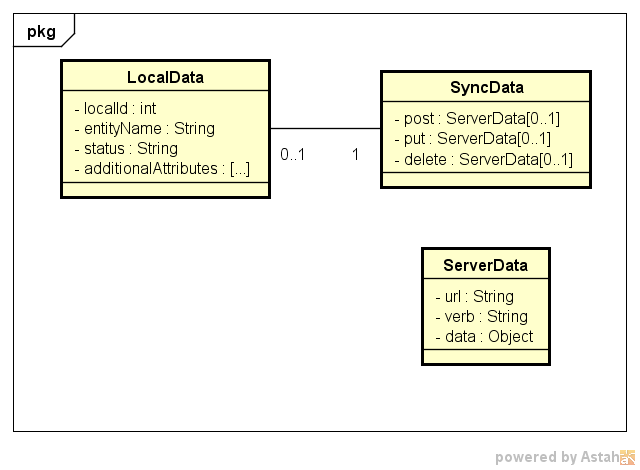
\includegraphics[width=0.8\linewidth]{content/images/DataModel-Cache-SPA}
\caption{Datenmodel zur Speicherung lokaler Daten}
\label{pic:DataModel-Cache-SPA}
\end{figure}

\subsubsection*{Umsetzung des Caches über HTTP-Verbs}
\label{sssec:Http-Verbs}
Durch diese Zentralisierung der Cache-Daten konnte ein Service entwickelt werden, der den \textit{\$http}-Service kapselt und bei jedem Senden einer GET-, POST-, PUT- und DELETE-Anfrage die lokalen Daten mit denen des Web Services synchronisiert. Dafür wird nach dem Senden der Nachricht geprüft, ob der Web Service erfolgreich erreicht wurde.\\
Ist dies der Fall, werden die neuen Daten mit dem Status \textit{server} lokal aktualisiert. Dies sagt aus, dass die Daten mit denen des Servers übereinstimmen und keine Synchronisation erfolgen muss.\\
Wenn der Web Service nicht erreicht wurde, werden die Daten mit dem Status \textit{local} zwischengespeichert. Dazu wird ein \textit{SyncData}-Objekt unterhalb des lokalen Datensatzes angelegt. Dieses definiert Eigenschaften mit Daten für spätere Synchronisationsprozesse.

\subsubsection*{Synchronisation zwischen Server und SPA}
\label{ssec:Sync-SPA}
Ist der Web Service wieder erreichbar, werden alle Datensätze mit dem Status \textit{local} synchronisiert, indem die Anfragen nacheinander an den Server gesendet werden. \\
Hierbei wird per Eigenschaft \textit{verb} entschieden, welche Methode des \textit{\$http}-Services genutzt werden soll. Dieser werden dann die gespeicherte URL sowie eventuelle Daten zum Senden an den Server übergeben. \\
Die Reihenfolge der verarbeiteten \ac{HTTP}-Verben für die Synchronisation wurde wie folgt gewählt:
\begin{itemize}
\item \textit{DELETE}\\
Besitzt ein Objekt eine DELETE-Eigenschaft, werden dessen Daten als erstes verarbeitet. Alle weiteren offenen Synchronisationsprozesse werden im Zuge der Löschung dieses Datensatzes ebenfalls mit gelöscht. Dadurch wird die Anzahl der benötigten Requests verringert. \\
Besitzt ein Synchronisationsobjekt sowohl eine POST- und DELETE-Eigenschaft, ohne, dass zwischenzeitlich eine Synchronisation durchgeführt wurde, ist das Objekt lokal erzeugt und anschließend wieder lokal gelöscht worden. Deshalb wird der Datensatz direkt aus dem lokalen Speicher entfernt, ohne, dass Anfragen an den Server gesendet werden müssen. Dies dient ebenfalls der Verringerung der zu sendenden Requests. 
\item \textit{POST} \\
Sind keine DELETE-Requests vorhanden, wird nach einem offenen POST- Request für das Objekt gesucht und bei Fund durchgeführt. Mit dem Ergebnis wird die ID des lokalen Datensatzes angepasst, damit eventuell anstehende PUT-Requests auf das richtige Server-Objekt angewandt werden.
\item \textit{PUT} \\
Zum Schluss wird auf offene PUT-Requests geprüft und gegebenenfalls durchgeführt. 
\end{itemize}
Nach jeder erfolgreichen Abarbeitung eines Synchronisationsbefehls wird dieser aus dem Synchronisationsobjekt entfernt. Wenn dieses daraufhin keine offenen Befehle mehr besitzt, wird es gelöscht. 
Damit der Nutzer nicht auf die Abarbeitung der Synchronisationsprozesse warten muss, wird dieser Vorgang komplett asynchron durchgeführt. Durch diese Änderungen ist eine Verbindung zum Web Service optional.

\subsection{Das AppCache-Manifest}
\label{ssec:appcache-manifest}
Der Einsatz des \textit{cachedHttpService} erlaubt eine Nutzung der \ac{SPA} auch ohne eine bestehende Verbindung zum Web Service. Doch noch braucht die \ac{SPA} eine Verbindung zum Web Server, damit statische Dateien wie View-Templates und Script-Dateien nachgeladen werden können. Diese Verbindungen können durch die Nutzung eines \textit{AppCaches} reduziert werden. \\
Der AppCache wurde im Zuge von \gls{HTML5} implementiert und wird von allen gängigen Browsern in der aktuellen Version unterstützt.\footcite{online:AngularJs:indexedDB:w3c}\footcite{online:caniuse:appcache} Hierbei wird eine Manifest-Datei auf dem Server abgelegt, welche Aussagen darüber trifft, welche Dateien lokal auf einem Client gespeichert werden sollen. Im Falle dieser Arbeit wurde konfiguriert, dass alle Dateien lokal gespeichert werden (siehe Code-Beispiel \ref{lst:SPA-appcache-manifest} ab Zeile \ref{line:appcache:local}ff.). 

\lstinputlisting[caption=Cache-Manifest-Datei, label=lst:SPA-appcache-manifest, style=htmlcssjs]{content/listings/CacheManifest.appcache}

Sind diese Dateien erstmal auf dem Client gespeichert, werden sie genutzt, wenn keine Verbindung zum Server besteht. \\
Damit die Dateien trotzdem auf dem aktuellen Stand sind, wurde im \textit{SETTINGS}-Bereich definiert, dass die Online-Ressourcen vorrangig genutzt werden sollen (siehe Zeile \ref{line:appcache:prefer-online}). Dies wird aber trotzdem nicht von allen Browser berücksichtigt. Deswegen gibt es eine Möglichkeit, den Client dazu zu zwingen  die Ressourcen erneut von Server abzurufen. Hierzu muss die Manifest-Datei angepasst werden. Wenn der Client das nächste Mal eine Verbindung zum Server aufbaut, wird die neue Manifest-Datei heruntergeladen. Dies für dazu, dass der Client alle lokalen Dateien invalidiert und sich die Dateien, welche das neue Manifest-Datei definiert, erneut herunterlädt. Damit das Aktualisieren der Datei leichter umgesetzt werden kann, wurde ein Zeitstempel als Kommentar in die Manifest-Datei integriert (siehe Zeile \ref{line:appcache:timestamp}). Somit kann man leicht ein Neuladen der Serverdateien herbeiführen. 
\section{Fazit}
Es konnte ein voll funktionsfähiger Prototyp entwickelt werden, welcher die vorher festgelegten Anforderungen umsetzt. Hierbei wurde der Funktionsumfang mit dem Browser \textit{Chrome} der Version 44.0.2403.157 getestet. \\
Vor- und Nachteile, welche sich durch während der Entwicklung der \ac{SPA} ergeben haben, werden gesondert in nachfolgende Kapitel \ref{cha:gegenueberstellung} beschrieben und bewertet. 

